\documentclass[../TV&MS.tex]{subfiles}
\begin{document}

\section{Условное математическое ожидание}

\subsection{Конструктивные определения}

\begin{Why}
    Уберите от экрана детей, беременных женщин и людей со слабой нервной системой.
Сейчас будем вводить условное математическое ожидание.
Для начала надо понять, а где тут вообще проблема и почему нельзя ввести условную плотность как отношение плотностей и тупо брать по ней интеграл.
Во-первых, что такое матожидание?
Матожидание - это простое обычное число.
А теперь рассмотрим две случайые величины: $\xi$ и $\eta$ и условное матожидание $\Expec(\xi|\eta)$.
Пусть для наглядности $\xi$ "--- число, выпавее на игральной кости, а $\eta$
"--- остаток от деления на $2$ выпавшего числа.
Тогда матожидание выпавшего числа будет равно $4$, если известно, что выпало
четное число, и $3$ "--- в противном случае.
То есть матожидание зависит от условия, которое является случайной величиной, 
а значит и само матожидание является случайной величиной.
Таким образом, условное математическое ожидание мы не можем тупо определить как интеграл от условной плотности, так как интеграл "--- это число.
Поэтому мы введем условное матожидание (УМО) отдельно для дискретных и непрерывных случайных величин, и в каждый раз будем вводить этого крокодила в $2$ этапа.
Сначала введем $\Expec(\xi | \eta = y)$ "--- матожидание относительно конкретной реализации случайной величины.
Это будет какая-то функция от $y$.
Потом скажем, что если в эту функцию подставить случайную величину $\eta$, то мы получим $\Expec(\xi | \eta)$ "--- УМО относительно случайной величины.
А потом еще для расширения сознания введем УМО относительно сигма-алгебры и введем все то же, но по-другому, аксиоматически, а не конструктивно.
\end{Why}

Пусть $\xi$ принимает значения $\{x_i\}$, а $\eta$ "--- $\{y_i\}$, тогда

\begin{Def}
    $
        \Expec(\xi | \eta = y_j) := 
        \sum\limits_{i} x_i \Pro(\xi = x_i | \eta = y_j) =
        \sum\limits_{i} x_i \dfrac{\Pro(\xi = x_i, \eta = y_j)}{\Pro(\eta = y_j)} = 
        f(y)$, \quad где $y = y_j.$
\end{Def} 

\begin{Def}
    $\Expec(\xi | \eta) = f(\eta)$, где $f$ "--- функция, полученная с помощью
    предыдущего определения.
\end{Def} 

Так как УМО "--- случайная величина, то мы можем взять матожидание этой 
случайной величины и посмотреть, а что будет.

\begin{multline}
    \forall B \in \Bor \quad
    \Expec\bigl[ \Expec(\xi | \eta) \Ind(\eta \in B) \bigr] =
    \sum\limits_{j\colon y_j \in B} f(y_j) \Pro \left( \eta = y_j \right) = \\
    = \sum\limits_{j\colon y_j \in B} \left[ 
    \sum\limits_{k} x_k \frac{\Pro \bigl(\xi = x_k, \eta = y_j\bigr)}{\Pro(\eta = y_j)}
    \right] \Pro (\eta = y_j) = \\
    = \sum\limits_{j\colon y_j \in B} \sum\limits_{k} \Pro\bigl(\xi = x_k, \eta = y_j\bigr) =
    \Expec\bigl[\xi \Ind (\eta \in B)\bigr].
\end{multline}

И в частности, если в качестве $B$ выбрать $\Real$, то индикатор всегда будет
равен 1 и тогда $\Expec\bigl[ \Expec (\xi | \eta) \bigr] = \Expec \xi$.

Теперь рассмотрим абсолютно непрерывные случайные величины
$\xi, \eta \sim p_{\xi, \eta}(x, y)$.
Попробуем подступиться так же, как и в дискретном случае, через условную вероятность.

\begin{equation}
        \Pro(\xi < x | \eta = y) = 
    \frac{\Pro(\xi < x, \eta = y)}{\Pro(\eta = y)} = \frac{0}{0}
\end{equation}

Проблемка. Попробуем тогда у условии сказать, что
$\eta \in [y, y + \varepsilon)$, и устремить $\varepsilon$ к нулю.

\begin{multline}
    \Pro \bigl(\xi < x | y \leqslant \eta < y + \varepsilon\bigr) =
    \frac{\Pro \bigl(\xi < x | y \leqslant \eta < y + \varepsilon\bigr)}
    {\Pro \bigl(y \leqslant \eta < y + \varepsilon\bigr)} = \\
    = \frac{\int\limits_{-\infty}^{x}\!\int\limits_{y}^{y + \varepsilon}
    p_{\xi, \eta}(x, y)dydx}
    {\int\limits_{y}^{y + \varepsilon} p_{\eta}(y)dy)} =
    \left\{ \text{\parbox{3.2cm}{считаем, что можно применить т. о среднем}} \right\} =
    \frac{\cancel{\varepsilon} \int\limits_{-\infty}^{x} p_{\xi,\eta}(x,y')dx}
    {\cancel{\varepsilon} p_\eta(y'')} = \\
    = \int\limits_{-\infty}^{x} \frac{p_{\xi, \eta}(x, y')dx}
    {p_\eta(y'')} \xrightarrow[\varepsilon \rightarrow 0]{} 
    \int\limits_{-\infty}^{x} \frac{p_{\xi, \eta}(x, y)}{p_\eta(y)}dx
.\end{multline}

Теперь можем вводить определение условной плотности:

\begin{Def}
    $p_{\xi | \eta = y}(x) = \dfrac{p_{\xi, \eta}(x,y)}{p_\eta(y)}$.
\end{Def} 

\begin{Wtf}
    Условная плотность "--- функция от $x$, но параметризованная $y$.
\end{Wtf}

\begin{Def}
    $\displaystyle \Expec(\xi | \eta = y) := \int xp_{\xi | \eta = y}(x)dx =
    f(y).$
\end{Def}

Теперь, как и в дискретном случае, конструктивно введем определение
УМО относительно случайной величины

\begin{Def}
    $\Expec(\xi | \eta) := f(\eta).$
\end{Def}
И снова посчитаем МО УМО:

\begin{multline}
    \forall B \in \Bor \quad
    \Expec\bigl[ \Expec(\xi | \eta) \Ind(\eta \in B) \bigr] =
    \Expec\bigl[ f(\eta)\Ind(\eta \in B) \bigr] =
    \int\limits_{B} f(y)p_\eta(y)dy = \\
    = \int\limits_{B}\!\int x \frac{p_{\xi, \eta}(x, y)}{p_\eta(y)}dx\ p_\eta(y)dy=
    \int\limits_{B}\!\int xp_{\xi, \eta}(x, y)dxdy = 
    \Expec\bigl[\xi \Ind(\eta \in B) \bigr]
.\end{multline} 

\subsection{Аксиоматическое определение}

Теперь потихоньку будем вводить УМО через всякие там приколы с мерой.
Вспомним наше любимое вероятностное пространство $(\Omega, \Ev, \Pro)$
и рассмотрим некоторую под"--~$\sigma$"--~алгебру $\mathcal{F} \subseteq \Ev$.

\begin{Def}
    Случайная величина $\eta$ называется \uline{$\mathcal{F}$"--~измеримой},
    если 
    $$\forall B \in \Bor \quad \eta^{-1}(B) = \bigl\{\omega\colon\eta(\omega) \in B)\bigr\} \in 
    \mathcal{F}.$$
\end{Def} 

\begin{Wtf}
    Поясним: рассмотрим игральную кость.
    Тогда $\Omega = \left\{ 1, \ldots, 6 \right\}$,\ $\Ev = \left\{ 2^{\Omega} \right\}$.
    Тепрь положим $\mathcal{F} = \bigl\{ \emptyset, 
        \left\{ 1, 3, 5 \right\},
        \left\{ 2, 4, 6 \right\},
        \Omega \bigr\}$.
    Теперь рассмотрим случайную величину $\eta$, которая равна чётности выпавшего числа.
    По определению легко проверяется, что $\eta$ является $\mathcal{F}$"--~измеримой.
\end{Wtf} 

\begin{Def}
    \uline{Условным математическим ожиданием} случайной величины $\xi$ 
    относительно $\sigma$"--~алгебры $\mathcal{F}$ называется случайная
    величина $\Expec(\xi | \mathcal{F})$, обладающая следующими свойствами:
    \begin{enumerate}
        \item $\Expec(\xi | \mathcal{F})\ \mathcal{F}$"--~измерима.
        \item $\forall A \in \mathcal{F} \quad 
            \Expec\bigl[ \Expec(\xi | \mathcal{F}) \Ind(A) \bigr] =
            \Expec \bigl[ \xi \Ind(A) \bigr]$
    \end{enumerate} 
\end{Def}

Введем теперь определение порожденной $\sigma$"--~алгебры.

\begin{Def}
    $\displaystyle \sigma(\eta) := 
    \bigcup\limits_{\forall B \in \Bor} \bigl\{\omega \colon \eta(\omega) \in B\bigr\}$
\end{Def} 

\begin{Wtf}
    Это объединение всех множеств, которые мы получили следующим образом:
    берем борелевское множество, смотрим, какие события туда <<попадают>>,
    если перегнать из событий в $\Real$.
\end{Wtf} 

И теперь, когда мы определили порожденную $\sigma$"--~алгебру,
можно вводить аксиоматические определения для УМО относительно случайных величин.

\begin{Def}
    $\Expec(\xi | \eta) := \Expec(\xi | \sigma(\eta)).$
\end{Def} 

Вообще по понятиям, если вводится такого рода определения, то надо доказывать корректность таких определений.
То есть мы определили какой-то новый объект, но еще не факт, что такие крокодилы водятся в природе.
Мы тут этим заниматься не будем, чтобы не опухнуть от функана.
Ключевые слова, чтобы казаться умным: мера, абсолютно непрерывная относительно другой меры, теорема Рад\'{о}на"--~Ник\'{о}дима, заряд.

\subsection{Свойства и красивые картинки}

Для начала запишем несколько свойств УМО (доказывать их я, конечно, не буду):
\begin{enumerate}
    \item $\forall B \in \Bor \quad \Pro\left( \xi \in B|\mathcal{F}\right)=
        \Expec\bigl[ \Ind(\xi \in B) | \mathcal{F} \bigr]$.
    \item $\Expec\bigl( a\xi_1 + b\xi_2 | \mathcal{F} \bigr) \Alsur
        a\Expec(\xi_1|\mathcal{F}) + b\Expec(\xi_2|\mathcal{F})$.
    \item Если $\eta\ \mathcal{F}$"--~измерима, то
        $\Expec(\xi\eta | \mathcal{F}) \Alsur \eta\Expec(\xi | \mathcal{F})$.
    \item Если $\xi$ и $\eta$ независимы, то
        $\Expec(\xi | \eta) \Alsur \Expec(\xi)$.
    \item $\Expec \bigl[ \Expec(\xi | \mathcal{F}) \bigr] = \Expec\xi$.
\end{enumerate} 

Теперь картинки. Мы придумаем какую-нибудь плотность $p_{\xi,\eta}(x, y)$, 
а потом построим график плотности условного матожидания и попытаемся понять
его жизненный смысл.

Чтобы было легко и просто мы представим плотность в таком виде:
\begin{equation}\label{gathEq}
    p_{\xi,\eta}(x,y) = p_{\xi|\eta}(x) p_{\eta}(y)
.\end{equation}

Затем положим:

\begin{equation}
     p_{\xi|\eta}(x) = \Norm(\eta, 1) = \frac{1}{\sqrt{2\pi}}
     exp\left\{ -\frac{(x-\eta)^2}{2} \right\}
,\end{equation}
\begin{equation}
    p_\eta(y) = exp(1) = e^{-y}\Ind(y \geqslant 0)
.\end{equation} 

Теперь по понятиям.
Что значит математическое ожидание $\xi$ при условии $\eta$?
Это МО, если считать, что $\eta$ уже свалилось к нам с неба и не меняется.
В силу построения условной плотности $\Expec(\xi | \eta) = \eta$ просто из свойства нормального распределения.
И полученная случайная величина, утверждается, что распределена экспоненциально.
Попробуем увидеть это на графиках.

\begin{figure}
\centering
\begin{minipage}[b]{0.5\textwidth}
    \centering
    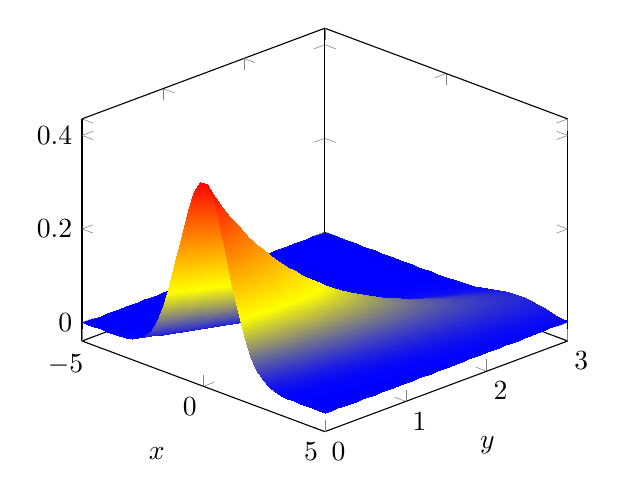
\begin{tikzpicture}
        \begin{axis}[view={45}{30},
            shader=interp,
            samples=40,
            domain y=0:3,
            xlabel=$x$,
            ylabel=$y$,
            ytick distance = 1,
            scale=.9]
            \addplot3[surf,
                domain=-5:5]
                {1/(sqrt(2*pi))*exp(-0.5*(x-y)^2 - y)};
        \end{axis} 
    \end{tikzpicture}
    \vfill
    \caption{Совместная плотность~\eqref{gathEq}.}
    \label{gathDensSide}
\end{minipage}%
\hfill
\begin{minipage}[b]{0.5\textwidth}
    \centering
    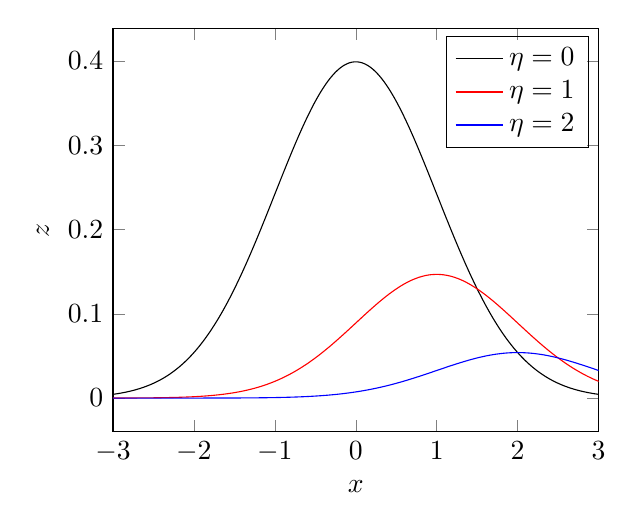
\begin{tikzpicture}
        \begin{axis}[
                ylabel=$z$,
                xlabel=$x$,
                xlabel style = {align=right},
                xmin=-3,
                xmax=3,
                mark=none,
                samples=300,
                scale=.9,
                legend entries = {$\eta=0$, $\eta=1$, $\eta=2$},
                legend style = {fill=none}
            ]
            \addplot[color=black]{1/(sqrt(2*pi))*exp(-0.5*x^2)};
            \addplot[color=red]{1/(sqrt(2*pi))*exp(-0.5*(x-1)^2 - 1)};
            \addplot[color=blue]{1/(sqrt(2*pi))*exp(-0.5*(x-2)^2 - 2)};
        \end{axis} 
    \end{tikzpicture}
    \vfill
    \caption{Сечения графика на рис.~\ref{gathDensSide} при различных реализациях $\eta$.}
    \label{cutsGathDens}
\end{minipage}
\end{figure}

Теперь если мы будем рассматривать сечения этого графика плоскостями
$y=t, t \geqslant 0$, то будем получать каждый раз почти графики плотности
нормального распределения с матожиданием $t$.
Почему почти? Потому что если проинтегрировать такой график, то получится
число, меньшее $1$, а именно равное вероятности (плотность имеет смысл
вероятности) того, что матожидание будет именно таким.
Так что в данном конкретном случае УМО можно увидеть на графике, рассматривая
сечения при различных $y$.
А вероятность попасть в то или иное УМО"---~это значение функции в максимуме
при конкретном значении $y$ с поправкой на множитель $\frac{1}{\sqrt{2\pi}}$. 
Если приглядется, то можно увидеть, что вероятность попасть в матожидание
убывает экспоненциально с ростом $y$, и так оно и должно быть в силу выбора
$p_\eta(y)$. 
Конечно, не всегда все так красиво, это просто жалкая попытка показать
на картинке жизненный смысл всего этого безобразия.


\newpage
\end{document} 
